INTRO

Google's T5 model, which is designed to perform well on data-scarce tasks. The results of a few experiments are reported, together with a brief summary of our findings.


FS
\subsection{Few-shot learning}
            Few-shot learning is a machine learning method used to generalise to a new task based on prior knowledge of other tasks \cite{wang2020generalizing}. It is mainly used when data for a specific task is scarce.
            
            A common way to approach few-shot learning consists in meta-learning a model to mimic few-shot learning scenarios. This is achieved through an episode-based training procedure \cite{NIPS2016_90e13578}. 
            
            For the task of few-shot text classification, \cite{geng2019induction} proposed the use of Induction Networks. An Induction Network is a Deep Learning architecture composed of a novel induction module that implements what is called a Dynamic Routing algorithm. This module enables the learning of generalized class representations, as opposed to static class representations that fail to generalize beyond training data.
            



METHOD
on two federated datasets for sentiment analysis. The first, Amazon Review \cite{yu2018diverse} has proven to perform well with few-shot learning and will be separated into nodes which each represent a device in a federated setting. The second, Sent140 \cite{caldas2019leaf}, is a federated dataset composed of Twitter comments, where each user corresponds to a node. We will use an Induction Network, which leverages meta-learning to carry out classification tasks.

Google's T5 model, which is designed to perform well on tasks for which data is particularly scarce. Our results will then be compared with the current benchmark for each dataset \textcolor{green}{\textbf{\cite{Bench1}}} \textcolor{green}{\textbf{\cite{Bench2}}}

    %\subsection{Induction Networks}
    %An Induction Network \cite{geng2019induction} is composed of three modules. The fist one is an encoder consisting of a bidirectional RNN with self attention. The second is an induction layer which enables the learning of generalized class representations.



DS
Sent140 \cite{caldas2019leaf} is a federated dataset whose tweets are automatically annotated based on the emoticons present in them. Each device is represented by a different twitter user.




            \subsection{Text-To-Text Transfer Transformer}
            Text-To-Text Transfer Transformer (T5) \cite{t5} is a language model with a text-to-text framework where the input consists in the description of the task and the data on which the task is to be carried out.
            
            \begin{figure}[h]
            \begin{center}
            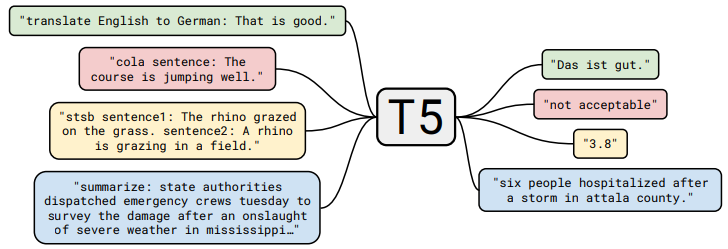
\includegraphics[width=\textwidth]{pics/T5.png}
            \caption{T5 input and output examples, as illustrated in the original paper \cite{t5}.}
            \label{fig:user}
            \end{center}
            \end{figure}
          
EXPERIMENTS
As the dataset contains 23 topics in total, 4 of which are reserved as a test set, we divided the remaining 19 topics into 3 groups which were used as separate nodes for training of the Induction model. The division has been done in the following way:
    \begin{itemize}
        \item First node (6 domains) - apparel, office products, automotive, toys games, computer video games, software;
        \item Second node (7 domains) - grocery, beauty, magazines, jewelry watches, sports outdoors, cell phones service, baby\footnote{"baby" domain was excluded from this node for testing the stacking approach};
        \item Third node (6 domains) - outdoor living, video, camera photo, health personal care, gourmet food, music.
    \end{itemize}
